\begin{figure}[h!]
  \centering
  \resizebox{\columnwidth}{!}{%
    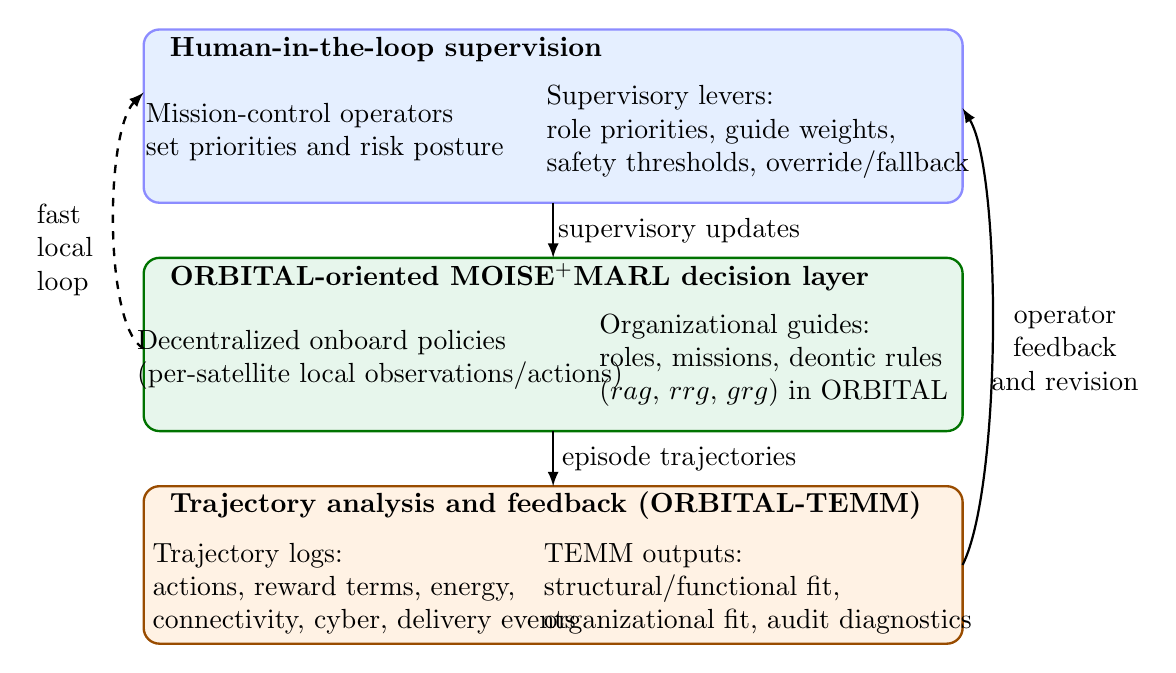
\begin{tikzpicture}[>=latex, line width=0.85pt]

      % Colors
      \definecolor{cTop}{RGB}{229,239,255}
      \definecolor{cMid}{RGB}{231,246,236}
      \definecolor{cBot}{RGB}{255,242,228}

      % Layer boxes
      \draw[rounded corners=2mm, fill=cTop, draw=blue!45] (0,5.6) rectangle (10.4,7.8);
      \draw[rounded corners=2mm, fill=cMid, draw=green!45!black] (0,2.7) rectangle (10.4,4.9);
      \draw[rounded corners=2mm, fill=cBot, draw=orange!60!black] (0,0.0) rectangle (10.4,2.0);

      % Titles
      \node[anchor=west, font=\bfseries\normalsize] at (0.2,7.55) {Human-in-the-loop supervision};
      \node[anchor=west, font=\bfseries\normalsize] at (0.2,4.65) {ORBITAL-oriented MOISE$^{+}$MARL decision layer};
      \node[anchor=west, font=\bfseries\normalsize] at (0.2,1.75) {Trajectory analysis and feedback (ORBITAL-TEMM)};

      % Top layer content
      \node[align=left, font=\normalsize] at (2.3,6.5) {Mission-control operators\\ set priorities and risk posture};
      \node[align=left, font=\normalsize] at (7.8,6.5) {Supervisory levers:\\ role priorities, guide weights,\\ safety thresholds, override/fallback};

      % Middle layer content
      \node[align=left, font=\normalsize] at (3,3.6) {Decentralized onboard policies\\ (per-satellite local observations/actions)};
      \node[align=left, font=\normalsize] at (8,3.6) {Organizational guides:\\ roles, missions, deontic rules\\ ($rag$, $rrg$, $grg$) in ORBITAL};

      % Bottom layer content
      \node[align=left, font=\normalsize] at (2.8,0.7) {Trajectory logs:\\ actions, reward terms, energy,\\ connectivity, cyber, delivery events};
      \node[align=left, font=\normalsize] at (7.8,0.7) {TEMM outputs:\\ structural/functional fit,\\ organizational fit, audit diagnostics};

      % Flow arrows (main loop)
      \draw[->, thick] (5.2,5.6) -- (5.2,4.9);
      \node[font=\normalsize, align=center] at (6.8,5.25) {supervisory updates};

      \draw[->, thick] (5.2,2.7) -- (5.2,2.0);
      \node[font=\normalsize, align=center] at (6.8,2.35) {episode trajectories};

      \draw[->, thick] (10.4,1.0) .. controls (10.9,2) and (10.9,6) .. (10.4,6.8);
      \node[font=\normalsize, align=center] at (11.7,3.75) {operator\\ feedback\\ and revision};

      % Fast local loop cue
      \draw[->, dashed] (0.,3.75) .. controls (-0.5,4) and (-0.5,6.5) .. (0,7);
      \node[font=\normalsize, align=left] at (-1,5) {fast\\ local\\ loop};

    \end{tikzpicture}%
  }
  \caption{Operational-assist architecture based on a ORBITAL-oriented MOISE$^{+}$MARL. Human supervision sets priorities and safety posture; decentralized policies are constrained by organizational guides; ORBITAL-TEMM analyzes trajectories and returns audit-oriented feedback for supervisory updates and corrective override.}
  \label{fig:operational-assist-architecture}
\end{figure}
